% \section{Experimental Results}
% \label{sec:exp-results}

% \subsection{Task 1: Cutting and pouring a package into a bowl}

% In this task, we tested our method on $n=6$ unique human participants in a mock apartment. Each trial took an average of 20-25 minutes, during which the robot acted in the vast majority of the time, and the human physically acted for roughly 15-30 seconds on average.

% The human participant was asked to sit on the couch and do their own work, and had the option to volunteer to get off the couch to perform more steps for the robot and/or agree/refuse the robot's help requests and task splitting proposals. The steps of the task were to (1) bring the bowl from the kitchen sink to the living room coffee table, (2) bring the package from the pantry shelf to the coffee table, (3) bring scissors, (4) use the scissors to open the package, and (5) pour the opened package into the bowl. Results are shown in Table~\ref{tab:real-world}.

\textbf{Experimental analysis.} Our experiments are designed to answer the following research questions:


\textbf{(1) Does our method achieve the best trade-off between task success and minimizing human effort?}
In our real-world user study (Table~\ref{tab:real-world}), \methodname{} achieves a 78\% task success rate compared to 28\% for the LLM baseline (statistically significant with $p$-value 0.007 under Fisher's exact test). Additionally, \methodname{} achieves a 94\% task step completion rate compared to the baseline's 58\% (statistically significant with $p$-value 0.002 under the Wilcoxon-signed-rank test). \ours{} understood its own limitations (through affordance functions trained in simulation), and was hence better at leveraging human assistance effectively on the steps it was ill-suited to perform.
The LLM baseline tended to prioritize minimizing human effort over task completion by allocating the robot multiple steps it was incapable of, since the LLM lacked an understanding of the robot's affordances.
Our method elicited more human effort than the baseline (40\% vs 18\%), so to control for the amount of human effort received, we compare our method to RECB in Figure~\ref{fig:rw-success-vs-human-effort}.
Despite RECB assuming oracle robot primitives and a perfectly cooperative human, our method still significantly outperforms it by more effectively balancing between success and human workload.

% Analyzing the results of our real-world user study in Tab.~\ref{tab:real-world}, we see that our method achieves a 61\% task success rate and completes 88\% of the plan steps with the human performing 38\% of these attempted steps. The pure LLM baseline, however, never managed to achieve any full task success, and was only able to complete 46\% of the plan steps in on average with the human performing 10\% of these attempted steps.

% The poor performance of the pure LLM baseline is primarily due to its difficulty in balancing the competing objectives of maximizing task success and minimizing total human effort.
% It frequently allocated infeasible tasks to the robot, even when provided with a list of feasible robot skills, often because it incorrectly judged the steps as semantically similar to a known skill.
% Moreover, the baseline tended to overemphasize minimizing human effort, making it overly reluctant to request human assistance even when necessary for successful task completion.

% While the pure LLM baseline achieved a much lower success rate than our method, it also received significantly less human assistance, primarily because it could not reliably determine when to request help.
% To control for human effort, we compare our method against RECB-1 and RECB-2 in Figure~\ref{fig:rw-success-vs-human-effort}.
% Despite our method experiencing failures due to imperfect action primitives, it still outperforms both baselines, which use the same amount of human effort but assume oracle primitives that never fail.

\begin{figure}[t!]
\centering
% \includegraphics[width=\linewidth]{figs/plots/combined_task_vs_effort.pdf}%
% \hfill%
% \includegraphics[width=\linewidth]{figs/plots/combined_task_vs_effort_sim.pdf}\\
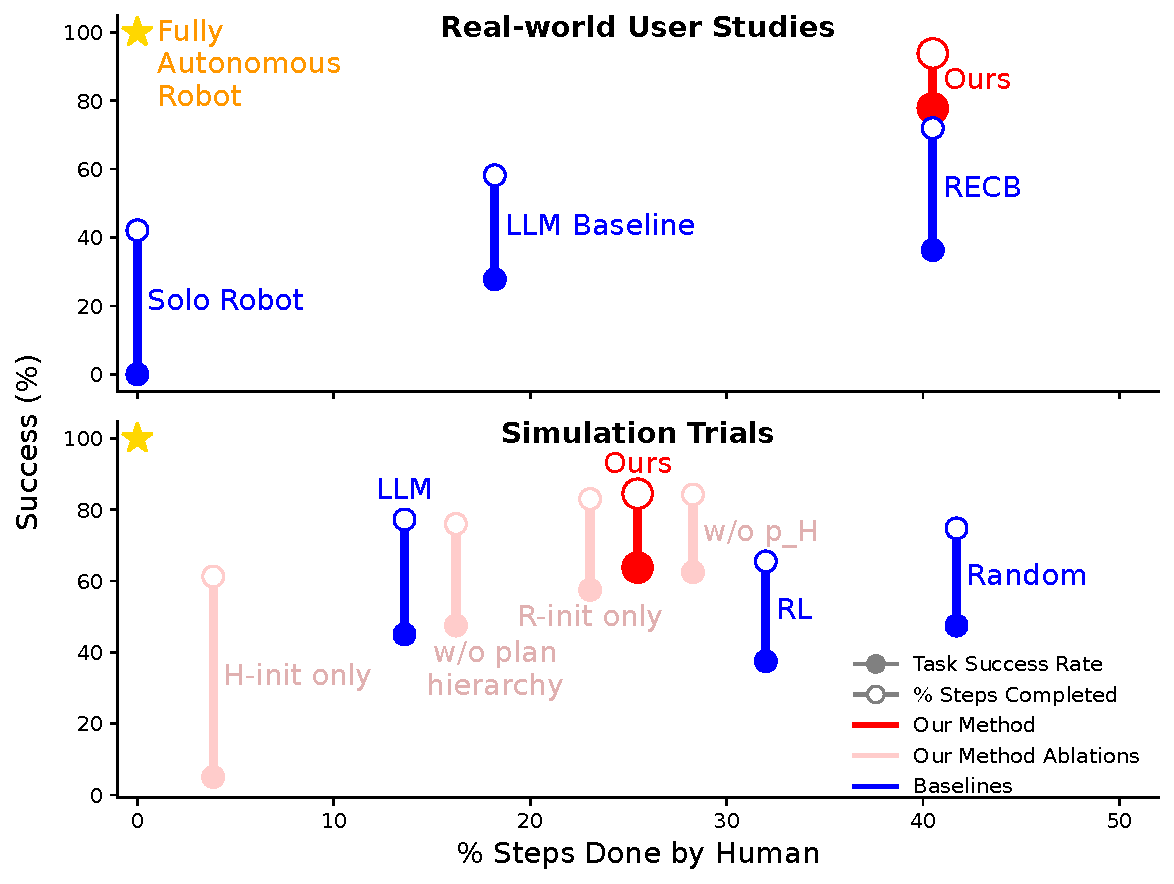
\includegraphics[width=\linewidth]{figs/plots/combined_task_vs_effort_real_sim.pdf}
\caption{In both \textbf{real-world} user studies \textbf{(top)} and \textbf{simulation trials} with a simulated human \textbf{(bottom)}, our method (red) demonstrates the best tradeoff in achieving task success (y-axis) for a given amount of human effort (x-axis) than baselines (blue) and our method's ablations (pink).}
\vspace{-3mm}
\label{fig:rw-success-vs-human-effort}
\end{figure}

\begin{figure}[t!]
    \centering
    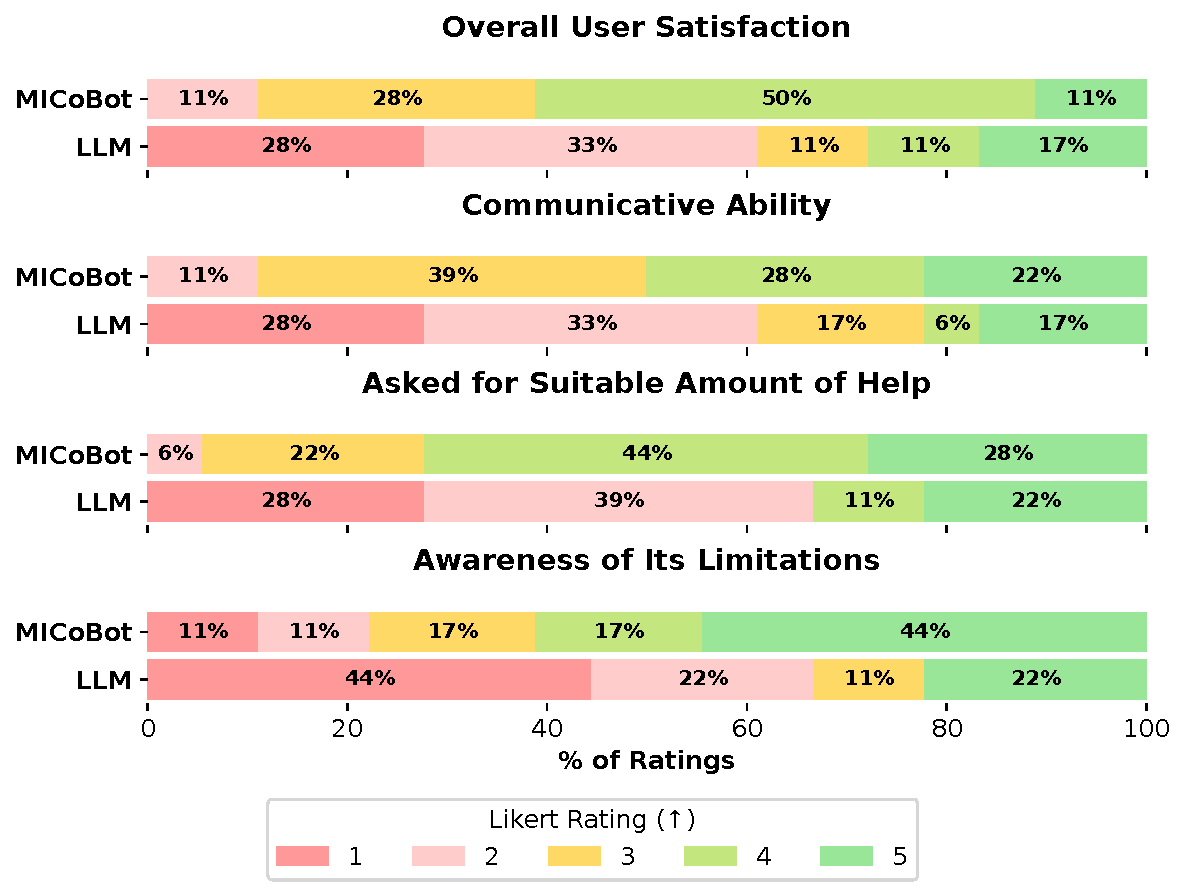
\includegraphics[width=\linewidth]{figs/plots/likert_plot.pdf}%\\
    \caption{\rev{Our method substantially outperforms the pure LLM baseline in user ratings averaged over all $n=18$ participants.}}
    \label{fig:likert-ratings}
\end{figure}

\textbf{(2) How do users feel about working with our system?
} The A/B blind preference test in Table~\ref{tab:real-world} shows that 78\% of users preferred our method over the LLM baseline.
% Among the three participants who favored the baseline, two experienced trials in which neither method completed the task, while the third preferred the baseline because it did not initiate conversation—unlike our method, which occasionally requested the user's assistance, even though the task ultimately succeeded.
Our method also significantly outperformed the baseline in user scores on overall satisfaction, \rev{communicative ability, and capability in asking for a suitable amount of help (statistically significant under the Wilcoxon-signed-rank test with $p$-values ranging from 0.007 to 0.024; see Figure~\ref{fig:likert-ratings}).} In contrast, the LLM baseline often failed to express when it needed help and was unwilling to reject human requests it could not fulfill, leading to over-promises and task failures. A representative dialog exchange, available
% Appendix Reference: in \ref{app:dialog-excerpt} and 
on our project site,\footnotemark[1]
% \href{https://mico-bot.github.io/user_study_dialog.html#user-study-1A}{website}
shows \methodname{} successfully persuading an initially reluctant user to perform a step the robot was incapable of executing.

% Our method also significantly outperformed the baseline in overall satisfaction, scoring 3.6 out of 5.0 compared to 2.2 for the LLM. Participants rated our system as more communicative (4.1 vs. 2.0), better at initiating dialog, and more aware of its own limitations. In contrast, the LLM baseline consistently failed to express when it needed help and was often unwilling to reject tasks it could not complete, leading to over-promises and task failures. A representative dialog exchange—available in the Appendix and on our project website—shows \methodname{} successfully persuading an initially reluctant user to perform a step the robot was incapable of executing.

% Our method achieved an average score of 3.6 out of 5 on the Likert scale for overall satisfaction in working with the robot, compared to 2.2 out of 5 for the baseline.
% This satisfaction gap was largest in Task 2 (assembling a toy car), where the human performed 60\% of the steps when collaborating with our method.
% Users likely rated our method more favorably because they perceived the robot as more communicative (3.5/5 for our method vs. 2.0/5 for the baseline) and better at initiating dialog, making it a more effective collaborator.

% Most users preferred working with our system not only because it achieved higher task success rates, but also because it was more grounded in the robot’s actual capabilities compared to the LLM baseline.
% Participants rated our method 4.1 out of 5 for clearly communicating when the robot was unable to perform a task, compared to 2.0 out of 5 for the LLM.
% The LLM, optimized through reinforcement learning from human feedback (RLHF) to prioritize user satisfaction, tended to eagerly agree to any human request, regardless of feasibility.
% As a result, some users felt the LLM was ``not cool'', criticizing it for making promises it could not fulfill.

\textbf{(3) Is mixed-initiative dialog critical to our method's performance?} Figure~\ref{fig:rw-success-vs-human-effort} (bottom) shows that our full method outperforms both ablated variants that restrict dialog to single-initiative modes: robot-only initiation (R-init) and human-only initiation (H-init). H-init performs especially poorly, as it prevents the robot from requesting help for steps it cannot execute. R-init performs slightly worse than the full method because it does not allow the human to proactively initiate dialog and assist when appropriate.
These results underscore the importance of mixed-initiative dialog in enabling flexible, robust human-robot collaboration.

% Appendix Reference: Additional experimental results and analysis (e.g. the role of $p_{H, t}$ estimation) are in \ref{app:extra-exps}.
% We ablate the $p_{H, t}$ estimator in our simulated experiments, fixing $p_{H, t} = 0.5$ for all timesteps and trials.
% We see from Figure~\ref{fig:rw-success-vs-human-effort} results in simulation (\texttt{w/o p\_help}) that being incapable of estimating the probability of human helping leads the robot to ask for help from the human more often (larger $x$-value), even when they are less likely to help overall (leading to no higher success rates on the $y$-axis).

In real-world user studies, \ours{} engaged in 2.4 dialog initiative shifts per trial, compared to the LLM baseline's 1.1. This enabled \ours{} to boost human acceptance of help requests from $55\%$ to $86\%$. The LLM baseline made far fewer help requests per trial (0.9 vs. \ours{}'s 2.9) and achieved a smaller acceptance increase ($70\%$ to $75\%$). This demonstrates mixed-initiative dialog is critical to collaborative discussion and task success.